The HPS experiment data acquisition and trigger system handles the acquisition of data and 
distribution of triggers for three sub-detectors; the SVT, ECal and the muon detector. There 
are two front end electronic systems; the SVT is readout with 128-channel integrated circuits
 supported by Advanced Telecom Communications Architecture~\cite{atca} (ATCA) hardware
 while the ECal and muon detectors signals are processed by VXS based hardware. The 
Level 1 trigger receives input from the ECal and muon detectors only to form a decision 
 on which events to be read out.  The triggered events are acquired from the three subsystems and are processed in the data acquisition system outlined in 
 Fig.~\ref{fig:daq_hardware_overview}.
\begin{figure*}[t]
%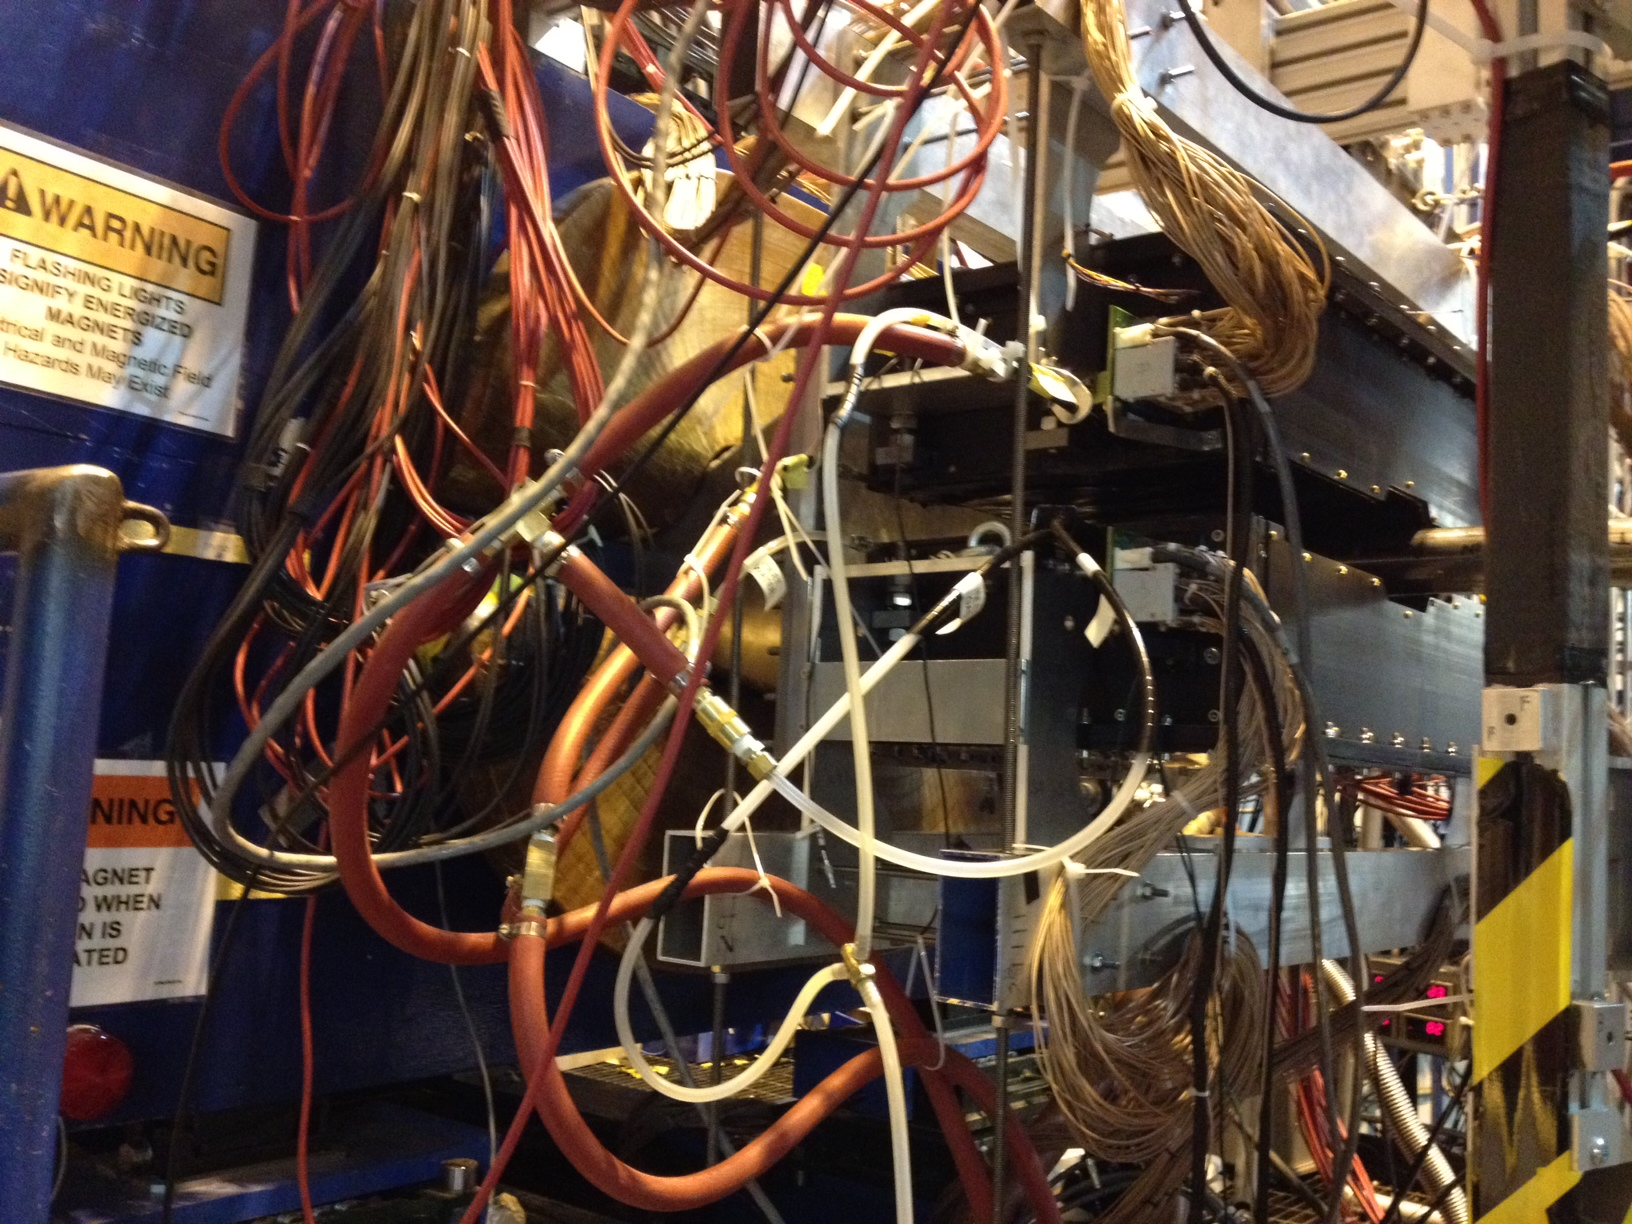
\includegraphics[ scale=0.25]{test2012/ecal_mounted.JPG}
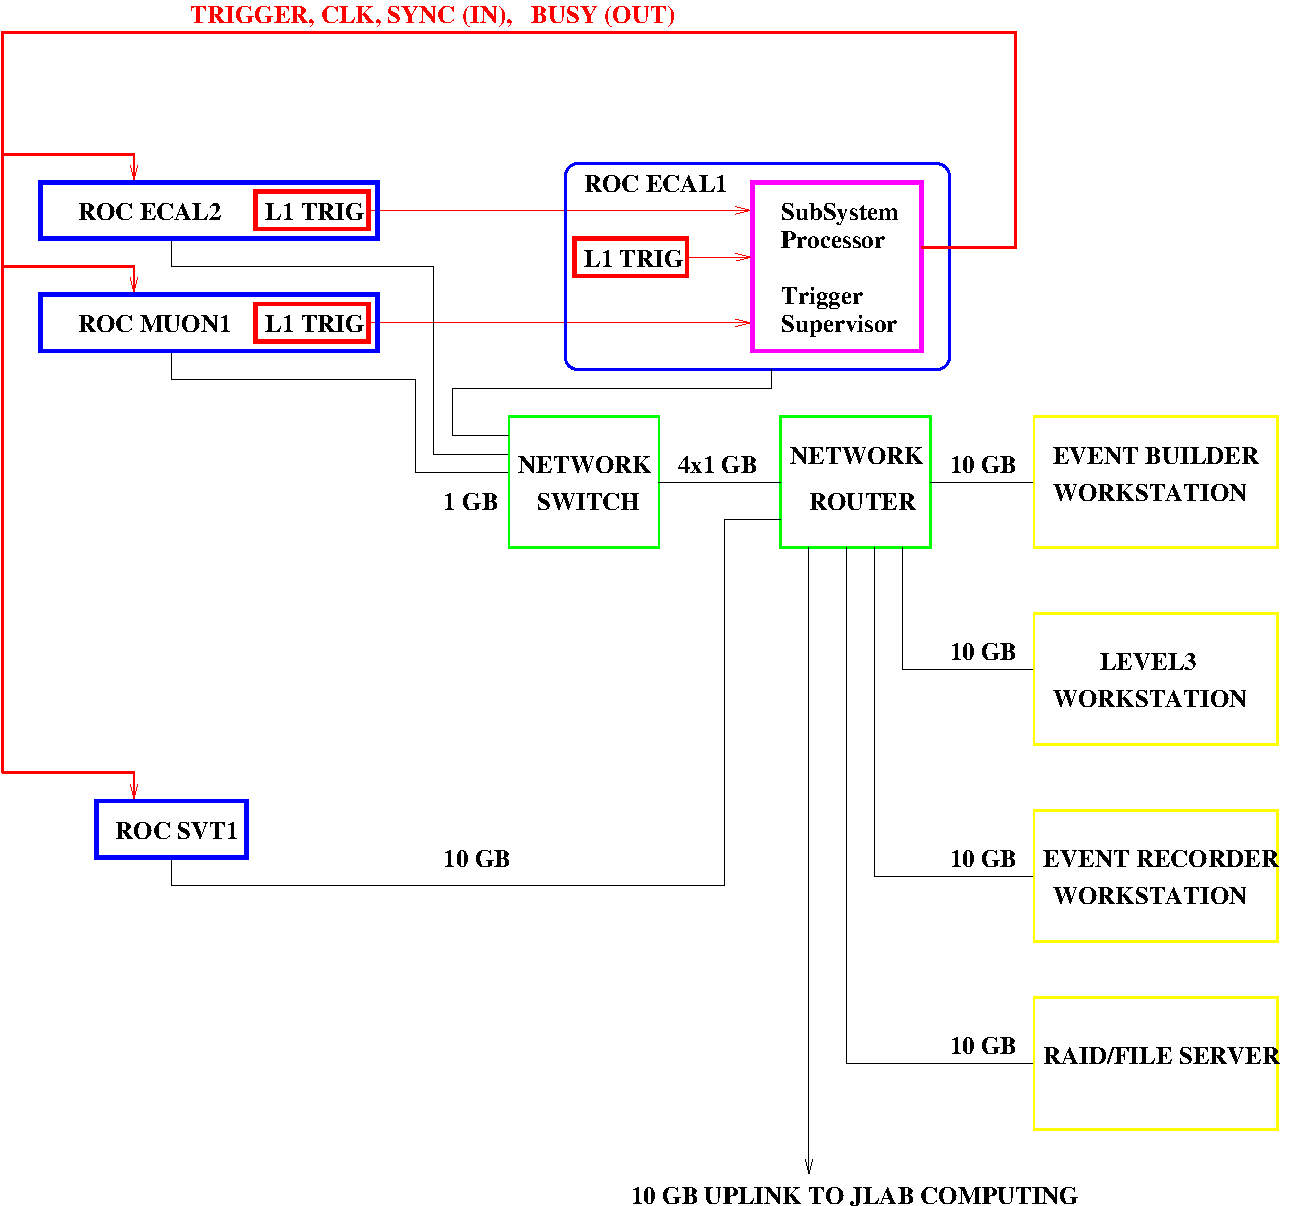
\includegraphics[ scale=0.3]{daq_trigger/figures/daq_schem.pdf}
\caption{\small{Schematic block diagram of the data acquisition system.}}
\label{fig:daq_hardware_overview}
\end{figure*}
Every VXS and VME crate contains the Readout Controller (ROC) that collects information 
from the front end electronics boards, processes it and sends it through the network to the 
Event Builder. ROC is the single blade Intel-based CPU module running DAQ software under CentOS Linux OS. The ROC for the SVT runs on 
a processor blade in the ATCA crate which handles the SVT part of the DAQ system. 
The Event Builder assembles 
information from the SVT, ECal and muon detector ROCs and assembles it into a single 
event which is passed to the Event Recorder which writes it to the data storage system capable of handling up to 100MBytes/s. The Event Builder and other 
critical components run on multicore Intel-based multi-CPU servers which is a 
sufficient configuration to handle HPS. The backbone of the DAQ network system is a 
Foundry router providing 1Gbit and 10Gbit connections between DAQ components and 
the JLab computing facility. The SVT ROC has a 10Gbit link to the Foundry router while the 
ROCs for the ECal and muon detector connect through a 1Gbit network switch. The long 
term data storage is handled by a 10Gbit uplink to the JLab computing facility. 

Section~\ref{sec:svt_daq} describes the SVT DAQ in more detail. The VXS based readout for 
the ECal and muon detector is described in Sec.~\ref{sec:fadc_daq} and the trigger 
system is explained in more detail in Sec.~\ref{sec:triggerdaq}.

\subsubsection{SVT Data Acquisition}
\label{sec:svt_daq}

\begin{verbatim}
This section needs update including optical readout and power distribution.
\end{verbatim}


The goal of the SVT DAQ is to support the continuous 40MHz readout and processing of signals from 
the 24 silicon strip sensors of the SVT and select those events that were identified by the 
Level 1 trigger system for transfer to the JLab DAQ for further event processing at rates 
close to 50kHz. 
Due to the difficult environment of the SVT with extreme occupancy and pile-up from multiple bunches  the number of noise hits has to be low to keep total data rates under control and 
each pulse from an energy deposition in the silicon needs to be sampled in order to facilitate 
reconstruction of the hit time to high accuracy. 

To meet these demanding requirements each of the 24 silicon strip sensors is connected to a 
hybrid board housing five 128-channel APV25~{\color{red}Reference needed} integrated circuits. The APV25, initially developed for the Compact Muon Solenoid silicon
 tracker~{\color{red}Reference needed}  at the Large Hadron Collider at CERN, was 
 chosen based on their good match to the HPS requirements. They provide amplification, 
 pipelining, and analog storage for trigger accepted events. For each 640-channel hybrid 
 board (shown in Fig.~\ref{fig:hybrid_and_apv25}
 \begin{figure*}[t]
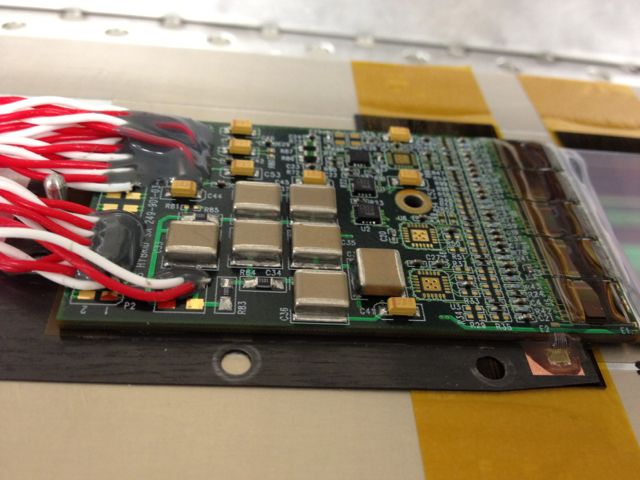
\includegraphics[ scale=0.3]{daq_trigger/figures/hybrid.jpg}
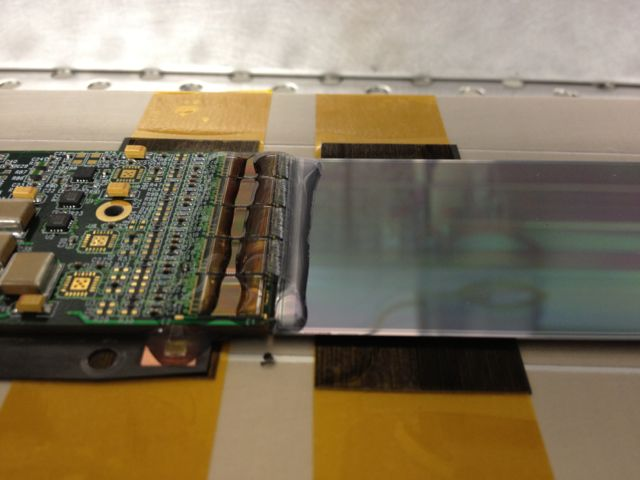
\includegraphics[ scale=0.3]{daq_trigger/figures/apvs-on-hybrid.jpg}
\caption{\small{Picture of a hybrid board from the test run in 2012 holding five 
APV25 ASICs that are wire bonded to the silicon sensor.}}
\label{fig:hybrid_and_apv25}
\end{figure*}
Each hybrid board has five analog output lines where analog data from each APV25 are 
sent using low power LVDS signals over about 3~m of multi-twisted-pair cable to a readout 
board. 

Figure~\ref{fig:svt_daq_overview} gives an overview of the SVT readout system. 
 \begin{figure*}[t]
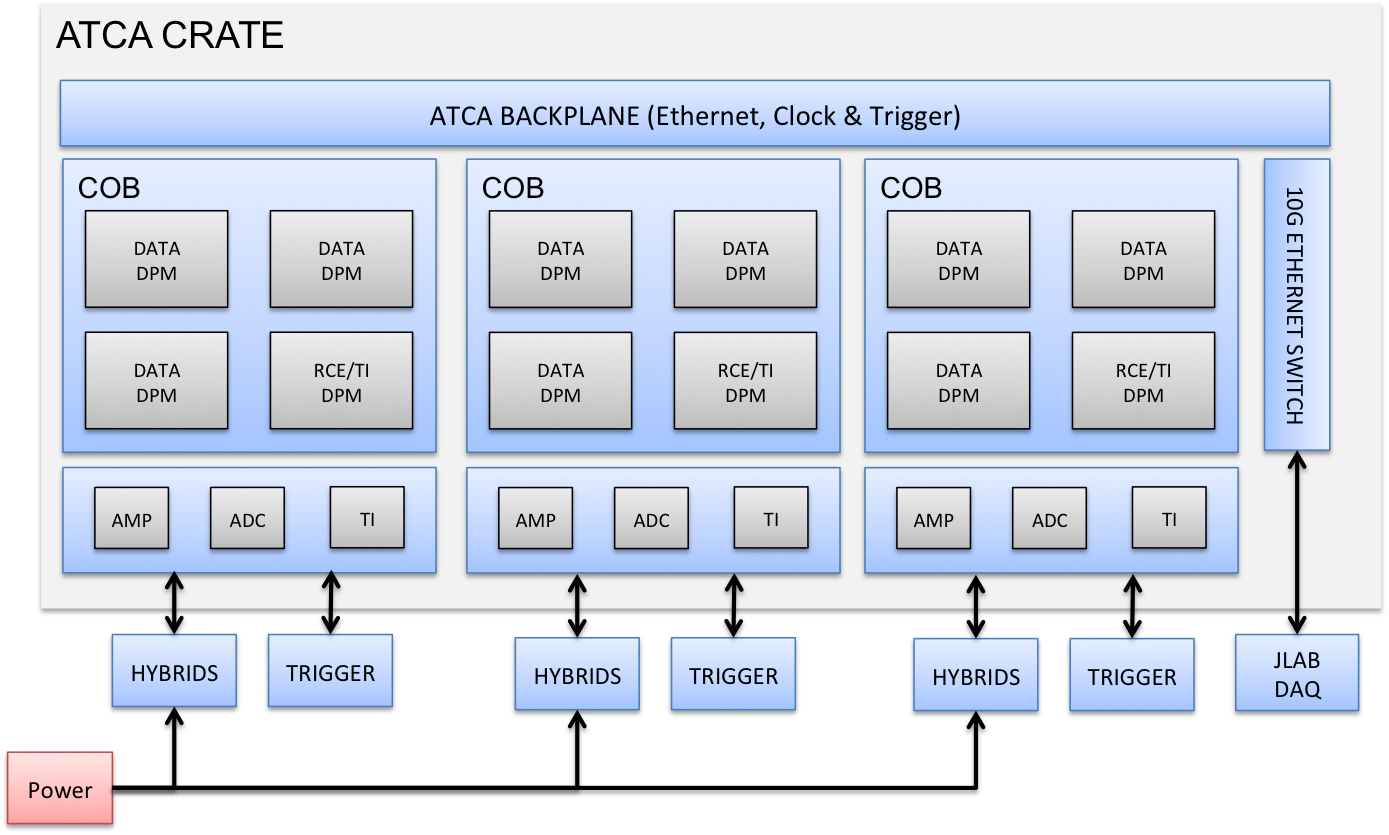
\includegraphics[ scale=0.6]{daq_trigger/figures/svt_daq_schem.png}
\caption{\small{Schematic block diagram of the SVT data acquisition system.}}
\label{fig:svt_daq_overview}
\end{figure*}
It is developed and built at SLAC using the Advanced Telecom 
Communication Architecture (ATCA) system for high speed data transfer. The analog signals 
from the 23,040 channels are digitized on the Rear Transition Module (RTM) boards. A 
pre-amplifier scales the APV25 differential current output to match the range of a 14-bit 
Analog to Digital Converter (ADC). Each RTM board has three sections that each service 
three hybrids. The ADC operates at the system clock frequency of 41.667~MHz. The RTM 
also has a 4-channel fiber optic module to communicate with the JLab trigger supervisor. 
A picture of a RTM board is shown in Fig.~\ref{fig:rtm}.
 \begin{figure*}[t]
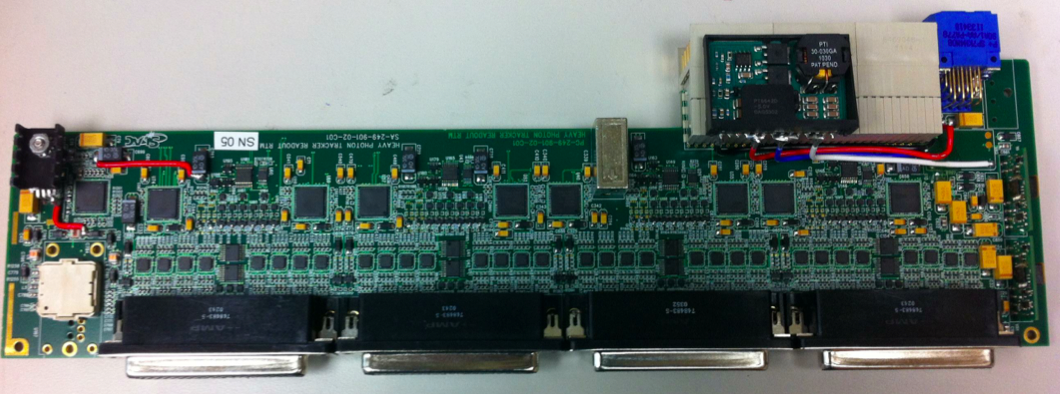
\includegraphics[ scale=0.25]{daq_trigger/figures/rtm.png}
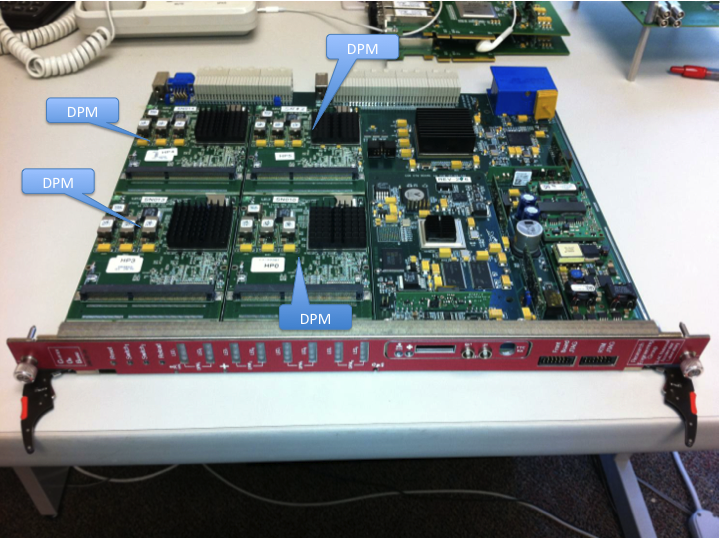
\includegraphics[ scale=0.4]{daq_trigger/figures/svt_daq_module_noted.png}
\caption{\small{Picture of a RTM (top) and COB board (bottom) 
used in the HPS test run 2012.}}
\label{fig:rtm}
\end{figure*}
The main COB board has four FPGA units that each interfaces with a single section of the 
the RTM.  Each FPGA is housed on a separate daughter board called 
Data Processing Module (DPM). Each DPM receives the digitized signals from the hybrids 
from the RTM, applies thresholds for data reduction and organizes the sample data 
into UDP datagrams. Each DPM also includes an I2C controller to configure and monitor the 
APV25 chips. One of the DPMs functions as the trigger interface which receives trigger 
signals from the optical fiber module on the RTM, handles distribution of clock and trigger 
and handles communication with the JLab trigger supervisor and the RCE. The 
RCE (Reconfigurable Cluster Element) is a generic computational building block 
on the trigger interface DPM running a 450~MHz PPC processor with 4GB of DDR3 
memory. Four COBs housed in a two ATCA crates is sufficient to handle 
the 36 hybrids of the SVT.

The RCE receives and buffers UDP datagrams from the data and trigger DPMs and
 assembles them into full event frames. The RCE also runs an implementation of the JLab ROC application that handles the integration of the SVT event frames into the JLab DAQ 
 system described above. The RCE node transfer data to the JLab DAQ  
 through a 10~Gbit Ethernet backend interface. 

The readout rate of the SVT is 43kHz, limited by the APV25 readout rate. 
%The maximum readout rate of the SVT DAQ  is limited by the readout time 
%of the APV25 chip. Using overlapping trigger and readout functionality, where the 
%APV25 chip can buffer up to 5 triggers, the maximum average readout rate expected for 
%HPS is 45kHz {\color{red} need verification}.   







\subsubsection{ECal and Muon Detector FADC Readout}
\label{sec:fadc_daq}
The main part of the readout of the ECal and muon detector are identical. Signals from each 
readout unit are sent to a signal splitter. For the ECal the charge signal from the APDs are 
shaped and amplified as described in Sec.~\ref{sec:ecal_readout} before feed into the 
splitter. One of the outputs of every splitter (for both the ECal and muon detector channels) 
feeds a separate channel on Flash ADC (FADC) readout boards that are packaged in 
16-channel VXS modules. Two 20-slot VXS crates are used to accommodate the two ECal 
halves, each one with 221 channels, and one 20-slot VXS crate is used to readout the muon 
detector. 

The FADCs stores the 12-but digitized samples of each channel in 8~$\mu$s deep pipelines. 
After a trigger is received a corresponding part of the pipeline is processed (usually few hundreds of nanoseconds). 
If the signal passes a predefined threshold, X number of samples before and Y samples after are summed. Transferring only 
the time it passed threshold and a channel sum as energy estimate greatly reduces the data rate. 
During data analysis value '(X+Y)*pedestal' will be subtracted to obtain actual pulse integral.

The FADCs are an integral part of the HPS calorimeter trigger system. Pulse energies 
and times from each FADC channel in the same VXS crate is collected by a crate trigger
 processor board (CTP) which performs cluster finding. The result from each create trigger processor (i.e. each half of 
the ECal) is combined in the sub-system processor module (SSP) which applies further selections 
based on single- and combination of clusters to form a trigger decision passed to the trigger 
supervisor. The trigger process has a pulse timing resolution of 4~ns. This allows a narrow 
coincidence window of 8~ns to be used when searching for clusters. 
This is an important part of improving 
the pattern recognition to reduce confusion in the tracker which has considerable longer 
integration times. 





The main characteristics of the Jefferson Lab Flash ADC are as follows:
\begin{itemize}
\item 12 bits digitizer with 250Msps
\item 50$\Omega$ termination input
\item Front-end input range  -0.5V, -1V or -2V.  Input range has to be above maximum pulse height to ensure no signal clipping
\end{itemize}

The FADC charge resolution as a function of the front-end input range is presented in Table~\ref{tab:charge_resolution}.
\begin{table}[h]
\centering
\begin{tabular}{| l | l |}
\hline
Input Range & Nominal Charge Resolution\\\hline
-0.5V & \ 9.76 fc per ADC count \\\hline
-1.0V & 19.53 fc per ADC count \\\hline
-2.0V & 39.06 fc per ADC count \\\hline
\end{tabular}
\caption{FADC charge resolution for different front-end input ranges.}
\label{tab:charge_resolution}
\end{table}

FADC data paths for the readout and trigger operation  are presented in Fig.~\ref{fig:hps_trigger_data}.
There are two FADC operation modes: the readout mode and trigger mode.

 In readout mode FADC determines the energy of the one ECal channel that will be reported. 
The channel integration occurs only if the input signal crosses the programmable threshold level.  Then a programmable number of samples around the threshold crossing are added together to form the reported integral.  The readout  mode has the following parameters for every FADC channel (see Fig.~\ref{fig:hps_trigger_data}, top panel):
 \begin{itemize}
 \item Number of samples integrated before the threshold crossing (NSB)
 \item Number of samples integrated after the  threshold crossing (NSA)
 \item Readout threshold, measured in ADC counts.
 \end{itemize}
 
The number of samples for a given channel integration  is the sum of NSB+NSA samples that will be stored in  
 the 17-bit FADC register. It is a fixed gate width pulse integration and there is no pedestal subtraction in the sum (pedestal subtraction happens offline).
 

 

\begin{figure}[t]
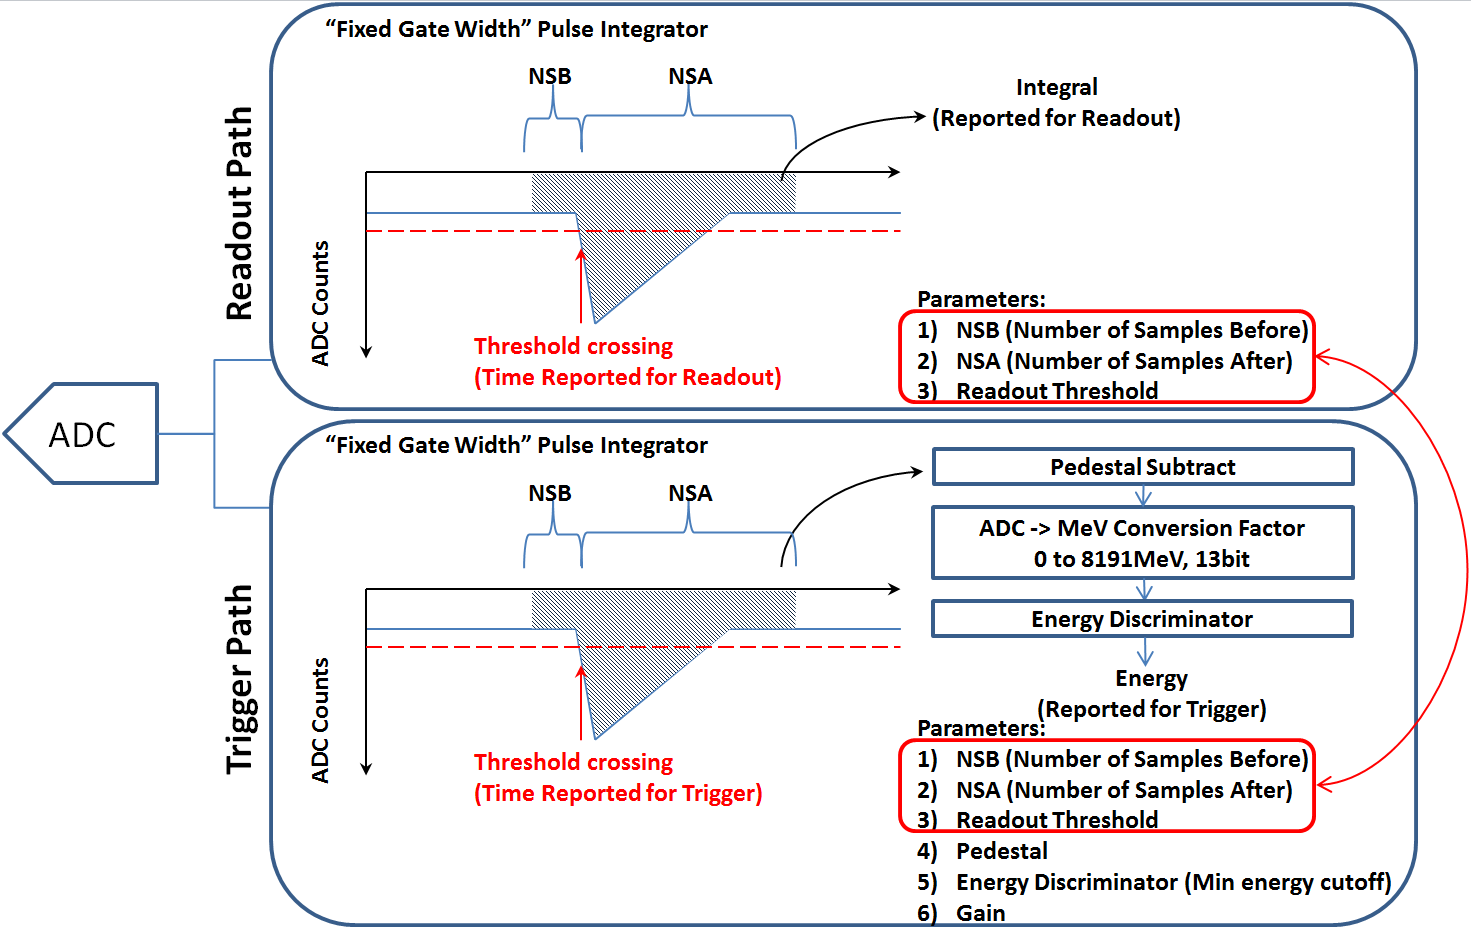
\includegraphics[scale=0.4]{daq_trigger/figures/hps_trigger_data}
\caption{\small{FADC data paths}}
\label{fig:hps_trigger_data}
\end{figure}

A block diagram of the HPS  trigger processing is shown in Fig.~\ref{fig:hps_trigger_data}, bottom panel. 
The trigger processing mode has the following parameters for every FADC channel:
 \begin{itemize}
 \item Number of samples integrated before the threshold crossing (NSB)
 \item Number of samples integrated after the  threshold crossing (NSA)
 \item Readout threshold, measured in ADC counts.
 \item Pedestal
 \item Conversion factor (gain) that converts  ADC channel to MeV, from 0 to 8191 MeV, 13 bits
 \item Energy discriminator (minimum energy cutoff)
 \end{itemize}
The parameters NSB, NSA and readout threshold are the same as in the readout mode.
The pedestal value is then subtracted from the integrated sum over NSB+NSA samples and this value is converted to MeV units using the gain conversion factor. The energy can be discriminated to cut off low energy pulses before reporting to the CTP. The value reported to the CTP is a 13bit pulse energy with a 4ns timing resolution where it crossed the readout threshold. Pulse data for every channel is sent to the CTP every 32ns (if there is no hit a 0 energy pulse is sent still). This sets a worst case double pulse resolution of 32ns per channel, but it can be as less than this if pulses occur in different 32ns windows, but close together).





See Sec.~\ref{sec:triggerdaq} for more details on the operation of the trigger system.


\subsubsection{Trigger System}
\label{sec:triggerdaq}

%\subsubsection{ECal Trigger overview}


The proposed trigger system is nearly deadtimeless. The trigger decision goes to the Trigger Supervisor every 4 ns. The trigger supervisor can apply deadtime if necessary, for example on a 'busy' or 'full' condition from front-end electronics.


\begin{figure}[t]
\includegraphics[scale=0.5]{daq_trigger/figures/FADC250_Photo_001.jpg}
\caption{\small{Jefferson Lab FADC250 VXS module.}}
\label{fig:fadc}
\end{figure}

The information from top and bottom parts of the ECal will be sent to the Jefferson Lab FADCs (Flash Analog-to-Digital Converters), Fig.~\ref{fig:fadc},  located in two different VXS crates (see Fig.~\ref{fig:hps_trigger_cal}). FADC  works at the frequency 250~MHz; i.e. it measures the amplitude of each ECal channel every 4 ns. FADC has 12bit pulse digitizer for readout and trigger processing. 

The first stage components of the trigger logic are incorporated into the Flash ADC board's FPGAs, while the final decision is made in a Crate Trigger Processors (CTPs) and  Sub-System Processor (SSP) .
FADC sends the information about the pulse energy and time to CTP.


\begin{figure}[t]
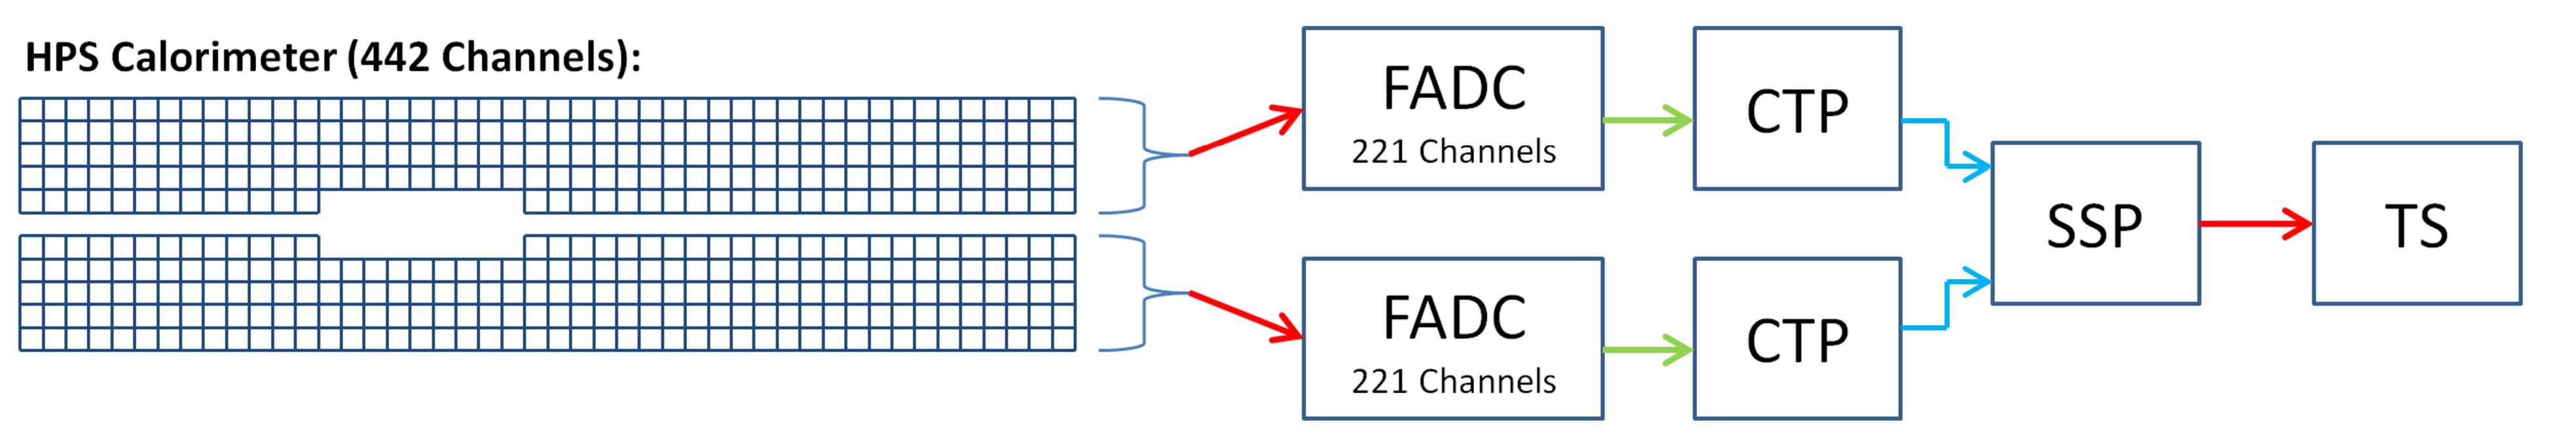
\includegraphics[scale=0.25]{daq_trigger/figures/hps_trigger_cal}
\caption{\small{ECAL trigger logic. FADC - Jlab Flash ADC, CTP - Crate Trigger Processor, SSP - Sub-System Processor, TS - Trigger Superviser.}}
\label{fig:hps_trigger_cal}
\end{figure}

The trigger system can be broken down into the following 3 sections:
 \begin{itemize}
 \item FADC (pulse finding): Samples the detector channel to find pulses. Pulse energy and times are sent to CTP.
 \item CTP (cluster finding): Searches FADC pulses (from half of calorimeter) to find clusters. Cluster energy, time, and hit pattern sent to SSP.
 \item SSP (cluster pair finding): Searches CTP clusters (from top and bottom) to find cluster pairs and create the trigger. Trigger cuts on pairs decide final trigger.
 \end{itemize}
 
 Trigger logic will search for a time coincidence between two clusters in opposite halves of ECal that occur within a programmable time window with 4ns resolution. The maximum trigger decision time (latency) is currently set to 3 $\mu$s for Level 1. That value is defined by the SVT readout APV25 chip.

The Trigger Supervisor generates all necessary signals, and controls the entire DAQ system readout through the Trigger Interface units. The Trigger Interface (TI) units installed in every crate participate in the readout process. The system is free-running and driven by a 250MHz global clock. The maximum trigger accept rate is 50 KHz.



%\subsubsection{Crate Trigger Processor} 

The Crate Trigger Processor receives the energy pulses (in MeV) and time stamp from each FADC channel in the crate (see Fig.~\ref{fig:hps_trigger_3x3}).
The algorithm used for cluster finding makes use the parallel processing nature of FPGAs by simultaneously searching for 125 clusters up to 3x3 in size across the calorimeter crystal array.  
A Cluster Processor (CP) algorithm:

\begin{itemize}
\item Add energy from hits together for every 3x3 square of channels in ECal
\item Hits are added together if they occur (leading edge) within a programmable number of clock cycles of each other (4 ns steps)
\item If 3x3 energy sum $\ge$  the programmable cluster energy threshold CTP reports cluster to the Sub-System processor the cluster parameters (time, energy, position and 3x3 hit pattern. 
\end{itemize}

Every 4ns the CTP evaluates all hits in its half of the calorimeter. A programmable time window is used to allow hits that are out of time with each other be considered as part of a cluster sum. This is done by reporting hits when they occur and then reporting them again for the next N number of 4 ns clock period, where N can be 0 to 7. This is useful to deal with skew and jitter that develop from the detector, cabling, and electronics.

When the sum of all hits in the 3x3 window occurring in a programmable time window are greater than the programmable energy threshold the cluster processor will report this cluster to the SSP if the energy is greater than all neighboring (up, down, left, right, and diagonals) 3x3 window cluster energies for that clock cycle. If the energy is not greater than its neighbor it will not be reported, but the neighbor will report if it is the greatest. The reason for this filtering is because there are several 3x3 windows that overlap and see the sample crystals and also many physics single clusters are larger than a 3x3 window.

The reported clusters to the SSP contain:

\begin{itemize}
\item 13bit Cluster energy (MeV)
\item Cluster position (crystal index: x,y)
\item Cluster time (4ns resolution)
\item Cluster hit pattern 3x3 (detector channels reporting a hit in the cluster)
\end{itemize}

The cluster position is the coordinate of the cluster processor that reported the cluster, which is where the peak cluster energy was seen from a 3x3 view. The 3x3 cluster hit pattern can be used by the SSP to help filter strange cluster patterns and/or make a low resolution cluster centroid computation.

\begin{figure}[h]
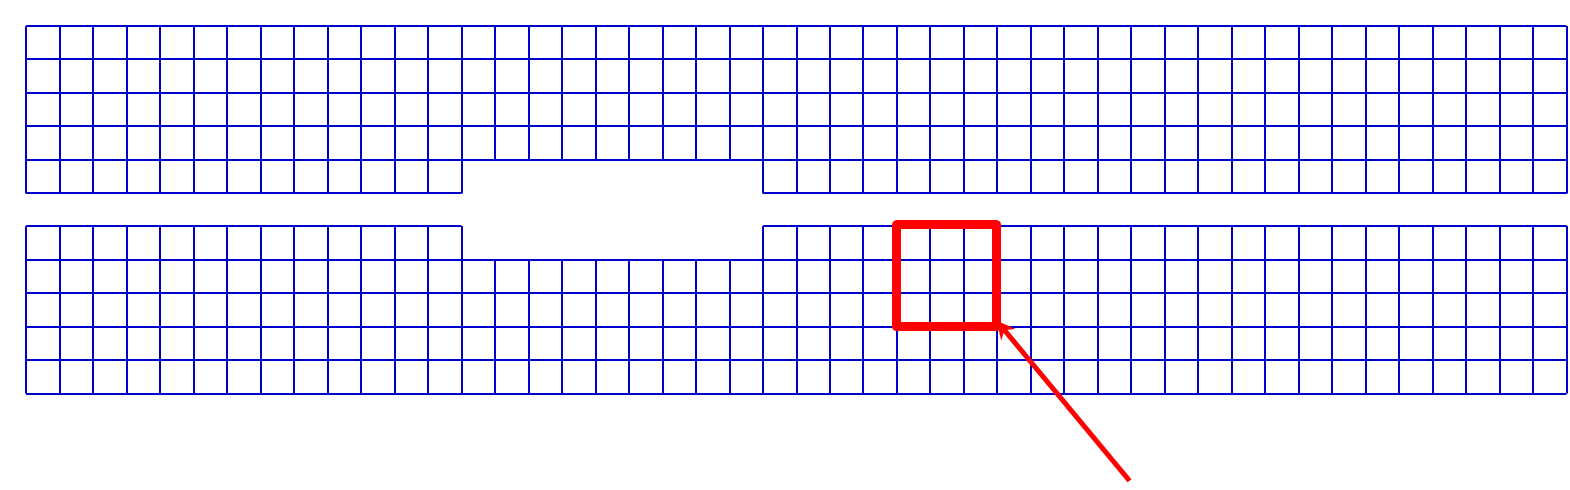
\includegraphics[scale=0.4]{daq_trigger/figures/hps_trigger_3x3}
\caption{\small{Cluster finding algorithm.}}
\label{fig:hps_trigger_3x3}
\end{figure}




%\subsubsection{Sub-System Processor} 

The cluster's time, energy, position and 3x3 pattern found in two VXS crates are reported to the Sub-System Processor. 
The SSP collects the cluster information from the full calorimeter and can create the trigger decisions of two types:
single cluster trigger and multi-cluster triggers.
Single cluster trigger condition includes the check on the cluster energy, $E_{min}\le E_{cluster}\le E_{max}$, where $E_{min}$ and $E_{max}$ are programmable minimum and maximum cluster energy.

Pairs trigger includes more conditions
\begin{itemize}
\item Energy sum,  
$E_{min}\le E_{top}+E_{bottom}\le E_{max}$
\item Pair time coincidence, 
$|t_{top}-t_{bottom}|\le \Delta t_{max}$ 
\item Energy difference, 
$|E_{top}-E_{bottom}|\le \Delta E_{max}$ 
\item Energy slope,
$E_{cluster\_with\_min\_energy}+R_{cluster\_with\_min\_energy}\times F_{energy}\le Threshold_{slope}$
\item Co-planarity, 
$|
tan^{-1}(\frac{X_{top}}{Y_{top}})-
tan^{-1}(\frac{X_{bottom}}{Y_{bottom}}) |\le Coplanarity_{angle}$
\item Number of hits in 3x3 window, 
\#$hits_{3\times 3}\ge HitThreshold$
\end{itemize}
\noindent
where $ E_{max}$,  $\Delta t_{max}$, $ \Delta E_{max}$ , $Threshold_{slope}$, 
$F_{energy}$, $Coplanarity_{angle}$
and
$HitThreshold$ are programable parameters.


Online event analysis will be provided to be compared against trigger event data for immediate verification (on each trigger cut: cluster energies, positions, timing, energy slope, coplanarity and hit threshold). With identical ADC readout and trigger pulse processing and high energy resolution, very precise agreement can be expected between trigger and readout.





%\subsubsection{Diagnostic Tools}

The previous experience with the similar (but much more simpler) trigger system showed that diagnostic tools are necessary to make sure that the calorimeter and trigger electronics work as expected. 

Scalers will be implemented for every ECal channel. The example of this diagnostic tool is presented in Fig.~\ref{fig:dvcs_beam}
from the previous version of the calorimeter. Hot or dead channels are easily identified online.
\begin{figure}[h]
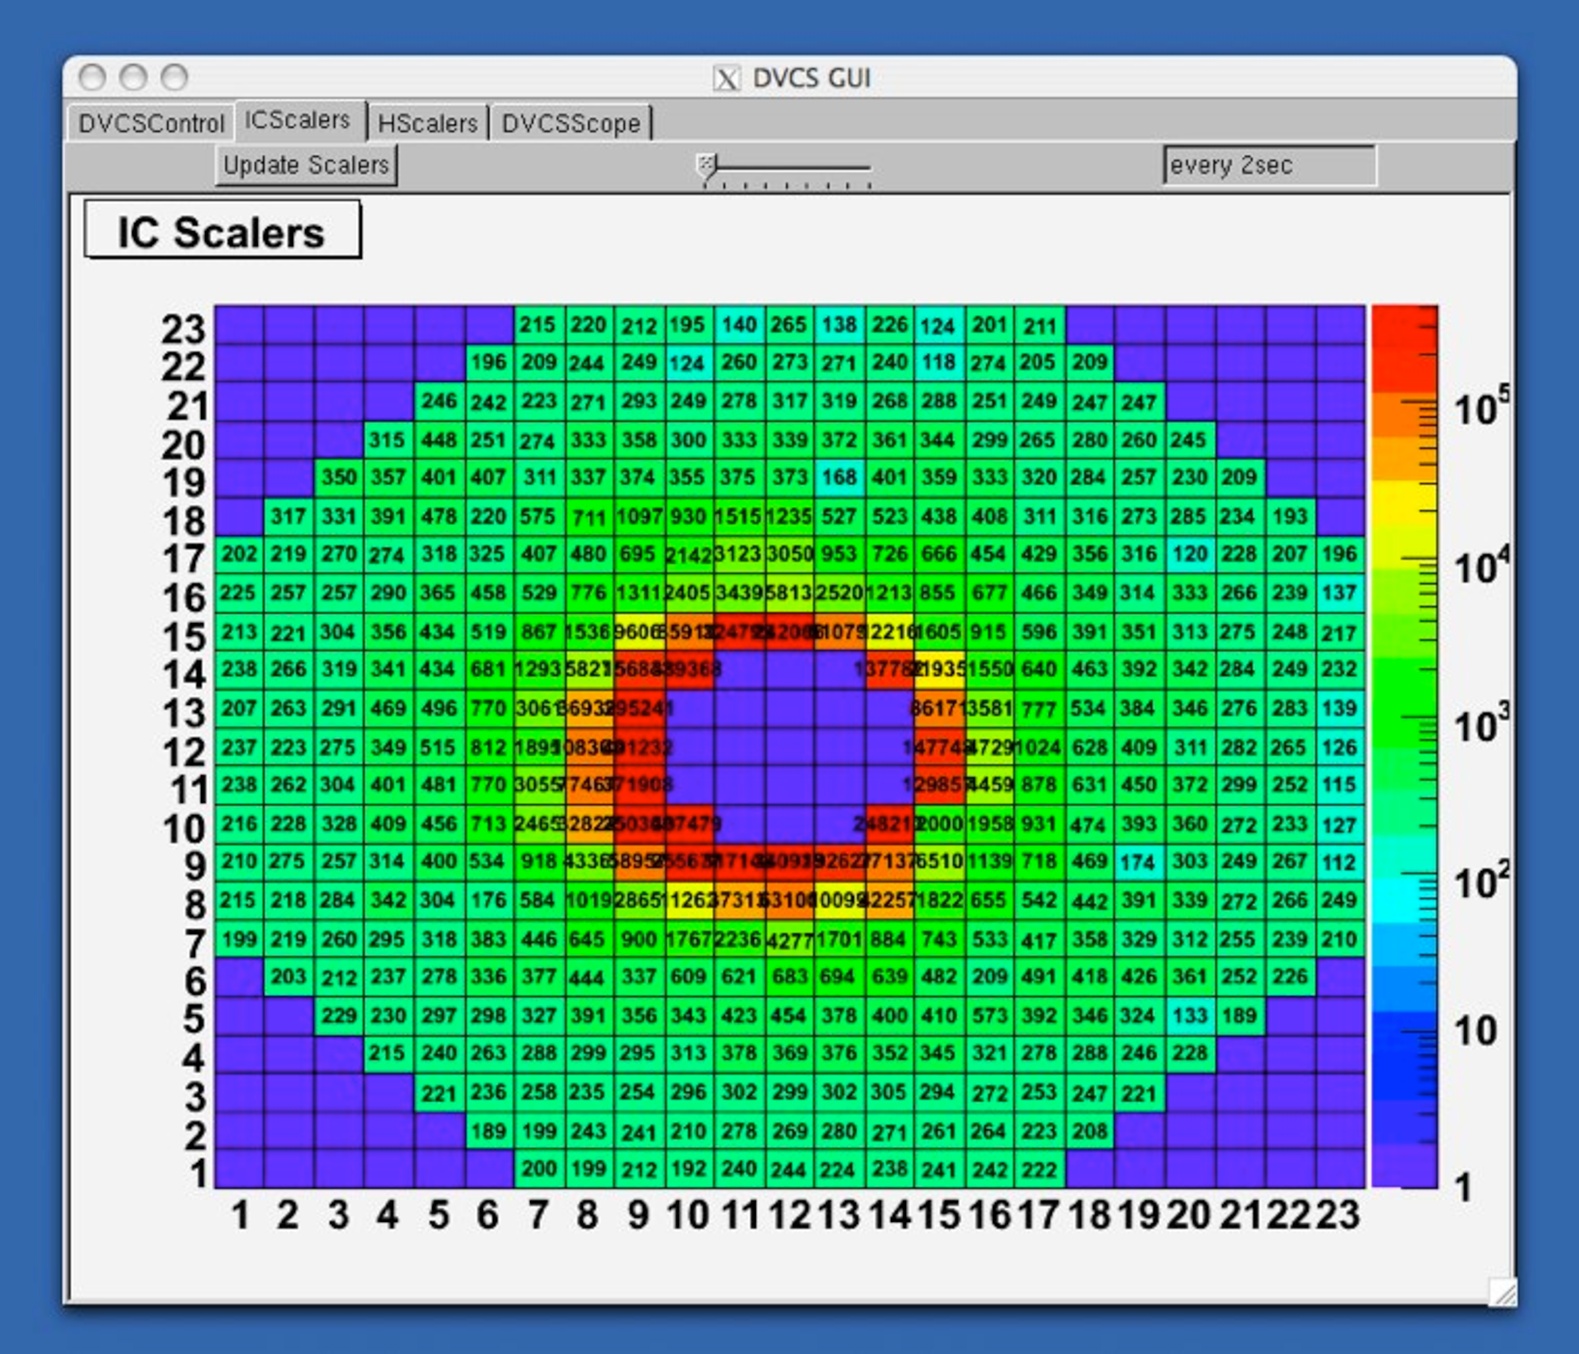
\includegraphics[scale=0.6]{daq_trigger/figures/dvcs_beam}
\caption{\small{Scalers (example from the previous version of the calorimeter).}}
\label{fig:dvcs_beam}
\end{figure}
Diagnostic scope permits to analyze on-line  the trigger logic. The goal to have  the Two-Dimensional Analyzer
 is to provide a remote debug interface to identify bad channels, verify cluster finding algorithms and check timing.
 The details of this analyzer are as following:
 
\begin{itemize}
\item Logic analyzer runs in parallel, non-intrusive, to the calorimeter trigger
\item Can setup trigger on any ECal pixel arrangement and/or cluster count
\item Can move forward/backward in time by ~250 ns to see timing details
\item Will be customize for HPS geometry and hardware
\end{itemize}

The example of the 2D analyzer is presented in Fig.~\ref{fig:dvcs_2_cluster}. Two clusters are displayed
in the picture. The red color displays the hits in the calorimeter and  the center of clusters is displayed in yellow.

In addition to the scalers, the distributions on individual ADC channel pulse energy will be provided.
The cluster hits positions and energy from SSP processor will be histogrammed as well. Two histograms (accepted and rejected) will be provided for each trigger cut used in the trigger logic.



\begin{figure}[t]
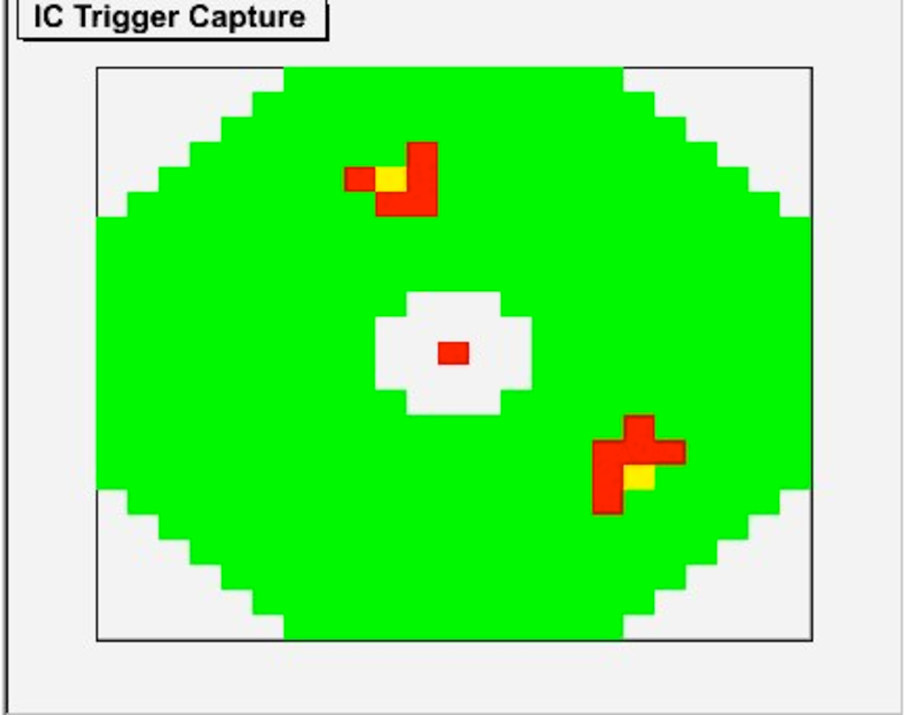
\includegraphics[scale=0.8]{daq_trigger/figures/dvcs_2_cluster}
\caption{\small{Diagnostic scope (example with two clusters found from the previous version of the calorimeter). Green - no hits, red - tower with hit, yellow - cluster found.}}
\label{fig:dvcs_2_cluster}
\end{figure}






%\subsubsection{Muon Trigger}

A muon detector composed of a four iron absorbers  and four double-layer scintillator planes, positioned after each absorber. Similar to the Ecal, the muon detector will consist of two halves, one above and one below the beam.
GEANT4 simulations have been used to study the trigger rates in the muon system due to background hits. It is expected that the true di-muon rate will be quite small compared to the ECal trigger rate and should not cause problem for the DAQ. 
A total of 144 readout channels are needed (9x16 channels multi-anode PMTs). Signals from each channel will be sent to a TDC and to a FADC. The FADC information will be used to construct the muon trigger. The TDC information together with information from FADC will be used in offline analysis to measure the hit position along the strip.

Selecting coincidence hits with MIP energy deposition in at least three layers of the scintillation hodoscope will identify muons. 
The muon trigger logic has to find one track in the top part of the detector in coincidence with another track in the bottom part of the detector. The track finding algorithm can be easily realized in the FPGA logic of the muon Crate Trigger processor.



\subsubsection{Event Size and Data Rates}

{\color{red}This needs to be updated with the latest occupancy values.}

The extreme radiation environment with tails of scattered beam imposing high occupancy
 puts strict requirements on high readout speed but consequently low noise readout to limit 
 the data rates. The event sizes and rates are based on estimates from detailed simulations 
 verified by measurements in the test run. 
  
As suggested in Sec.~\ref{sec:svt_desc}, the SVT will be operating at an effective threshold of three
times the noise level or an equivalent of 0.135\% occupancy. This translates to on average of 21 channels above threshold. Background studies (see Sec.~\ref{sec:hps_perf}) show that 
there are on average 10 tracks per event at a beam energy of 2.2~GeV and current of 
200~nA. With each track 
having on average 2 strips above threshold for each sensor there are on average 160 channels above threshold. Each of these channels will result in six digitized samples of the 
pulse shape giving in total of 1084 samples per event for the SVT.
Each channel has, in addition to the digitized samples,  header information that identifies the 
the channel number and it's chip address. The complete SVT event size also 
include the overhead from each FPGA and the JLab data stream bank header.  
With the average occupancy 
estimated above the expected event size is 3.6~kbytes corresponding to a data rate of 
approximately 155~Mbytes/s assuming an average trigger rate of 43~kHz.  
This high data rate is handled utilizing 
the 10~Gbit ethernet connections internally of the ATCA crate and also to the JLab DAQ.
{\color{red} (need to update these with the exact simulation of environment}


The data rate from the ECal and muon system is estimated from the same running 
conditions as the SVT above. 
Each calorimeter or muon hit consist of 8 bytes (4 byte energy, 4 byte time)
 with a 12 byte header (4 byte trigger number, 8 byte trigger time) for each FADC board. 
 The main limitation is of the order of 100Mbytes/s from each VXS crate. For a 
 10\% occupancy estimated in Sec.~\ref{sec:trig_rate} the ECal event size is approximately 0.7~kbytes which translates to a total data rate of approximately 31.5~Mbytes/s 
(split between the two VXS crates), well within the DAQ system design. 

The contribution from the muon system is small due to it's significantly lower number of channels. The system is readout by nine FADC boards in a single VXS crate. The event 
size for a 10\% occupancy level is 0.2~kbytes which translates to a data rate of 10~Mbytes/s. 

Table~\ref{tab:data_rates} summarizes the event size and data rates for the different 
sub-systems. 
\begin{table}[]
\centering
\begin{tabular}{l|c|c|c}
Sub-system & Occupancy(\%) & Event size (kB) & Data Rate (MB/s) \\
\hline
SVT & 0.135 & 4.5 & 203 \\
ECal & 10 & 0.7 & 32 \\
Muon & 10 & 0.2 & 10 \\
\hline
Total & - & 5.4 & 245 \\
\hline
\end{tabular}
\caption{{\small Occupancy, event size and data rate expected for beam energy of 2.2~GeV and a current of 200nA.} {\color{red}Need update}}
\label{tab:data_rates}
\end{table}
The dominant contribution comes from the SVT where irreducible real hits from the high occupancy is dominating the rates. Using high-speed data links it's still within the DAQ system and high performance file servers it's within the the system design. 

The total data volume for a 2 week long production run is expected to be around 83Tb 
assuming a duty factor of 30\%.  For a longer run a Level~3 fast track trigger can 
be deployed to lower the data rates and total volume to be written to disk. 
